\section{Introduzione agli agenti intelligenti}
Parte di questo documento fa riferimento ai lucidi del corso che sono parzialmente basati sul libro di testo del corso “M. Wooldridge, An Introduction to Multi-Agent Systems, Wiley, 2009” e sul materiale fornito da Alberto Martelli dell’Università degli Studi di Torino.

\subsection{La Computazione}
Prima di introdurre gli agenti intelligenti sarà utile discutere dei cinque trend che hanno caratterizzato la storia della computazione, ovvero:
\begin{itemize}
    \item Ubiquità: La continua riduzione dei costi di elaborazione ha permesso la diffusione di sempre più dispositivi.
    \item Interconnessione: I sistemi informatici oggi non esistono più da soli, ma sono collegati in rete in grandi sistemi distribuiti, quindi sono sempre più interconnessi (e.g. LAN, Internet, ...)
    \item Intelligenza e Delega: I computer fanno di più per noi, senza un nostro intervento (e.g. sistemi a guida autonoma, ...)
    \item Human Oriented: Spostarsi da una vista orientata macchina della programmazione verso concetti e metafore che sono più vicine al modo con cui noi comprendiamo e vediamo il mondo, quindi l'utilizzo di astrazioni più familiari per l'uomo (e.g. Object Oriented Programming per gli sviluppatori)
\end{itemize}

Delegazione e intelligenza implicano la necessità di \textbf{costruire sistemi informatici in grado di
agire efficacemente per nostro conto}.
\begin{itemize}
    \item La capacità di agire dei sistemi informatici in modo \textbf{indipendente}
    \item La capacità dei sistemi informatici di agire in un modo che \textbf{rappresentino nel migliore dei modi i nostri interessi} durante l’interazione con altri esseri umani o sistemi
        \begin{itemize}
            \item Interconnessione e distribuzione, accoppiate con la necessità di sistemi che rappresentino nel migliore dei modi i nostri interessi, portano a sistemi che possono
cooperare e raggiungere accordi o competere.
        \end{itemize}
\end{itemize}

Tutte queste tendenze hanno portato alla nascita di un nuovo campo in informatica: \textbf{Sistemi multi-agente}.

\subsection{Gli Agenti}
Un \textbf{agente} è un sistema di computazione capace di agire in modo \textbf{indipendente} per conto di un utente o proprietario, capendo cosa deve essere fatto per soddisfare gli \textbf{obiettivi} di progettazione, piuttosto che essere costantemente informato.

Un \textbf{sistema multi agente (MAS)} consiste in una serie di agenti, che interagiscono l’uno con l’altro. Per interagire con successo, richiedono la capacità di \textbf{cooperare}, \textbf{coordinarsi} e \textbf{negoziare} tra loro, in modo analogo a quanto fanno le persone. Un MAS quindi ha il compito di rispondere a queste domande:
\begin{itemize}
    \item Come possiamo creare agenti capaci di agire in modo indipendente, autonomo, in
    modo che possano svolgere con successo i compiti che gli deleghiamo?
    \item Come possiamo creare agenti capaci di interagire (cooperare, coordinare,
    negoziare) con altri agenti con il fine di portare a termine con successo i compiti
    delegati, soprattutto quando non si può presumere che gli altri agenti condividano
    gli stessi interessi/obiettivi?
\end{itemize}

Il primo problema è di progettazione/design di un agente, quindi micro, il secondo `e di progettazione/design di una società di agenti, quindi macro.

\subsection{Esempio: Curiosity}
Curiosity è un rover robotico delle dimensioni di un’auto che esplora il cratere Gale su Marte come parte della missione Mars Science Laboratory (MSL) della NASA. Curiosity è stato lanciato da Cape Canaveral il 26 novembre 2011.

Gli obiettivi del rover includono: indagini sul clima marziano e geologia; valutazione del fatto che il sito selezionato offra condizioni ambientali favorevoli per vita microbica, inclusa un’indagine sul ruolo dell’acqua; etc.

\textbf{Curiosity ha operato in modalità autonoma per circa 25 giorni.}

Per far ciò si è deciso di basare la sonda su \textbf{algoritmi di pianificazione} e non solo su sistemi di controllo ingegneristici.

\subsection{Caratteristiche degli Agenti}
In ultima istanza possiamo vedere un agente come un \textbf{sistema di computazione} capace di agire \textbf{autonomamente}, in maniera indipendente e in modo \textbf{flessibile}, in un qualche \textbf{ambiente} con il fine di raggiungere gli \textbf{obiettivi} per cui è stato progettato.

\begin{center}
    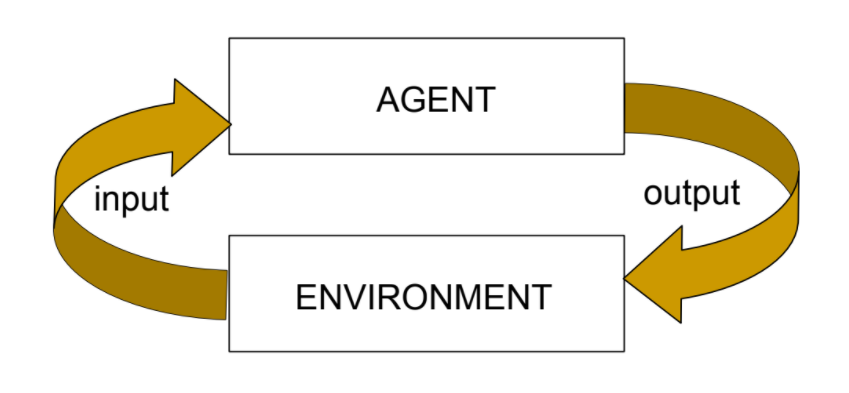
\includegraphics[scale=0.4]{images/agente_ambiente.PNG}
\end{center}

Un esempio di agente intelligente triviale, quindi banale, non interessante, è il termostato. Infatti il termostato decide cosa fare, ovvero accendere, spegnere il riscaldamento o non fare nulla, sulla base della temperatura rilevata dall'ambiente.

\subsection{Flessibilità}
Come anticipato nel precedente paragrafo un agente intelligente è un sistema di computazione capace di esibire azioni autonome in modo \textit{flessibile} in un ambiente. Con flessibile si intende:
\begin{itemize}
    \item Reattivo
    \item Proattivo
    \item Sociale
\end{itemize}

\subsubsection{Agente Reattivo}
Un agente reattivo è un sistema che mantiene una costante interazione con l’ambiente e risponde ai cambiamenti che occorrono su di esso (in tempo perché la risposta sia utile).
Bisogna tenere a mente però che l'ambiente reale è dinamico e le informazioni a volte possono essere incomplete.

Un agente reattivo può essere implementato tramite semplici regole condizionali del tipo: \textit{“if car-in-front-is-braking then initiate-braking”}, se l’agente percepisce che l’auto di fronte sta frenando, allora inizia immediatamente a frenare per evitare una possibile collisione, senza perdere tempo a ragionare, in sintesi quello che viene fatto è, per dato evento/stimolo → una regola di risposta.
\begin{center}
    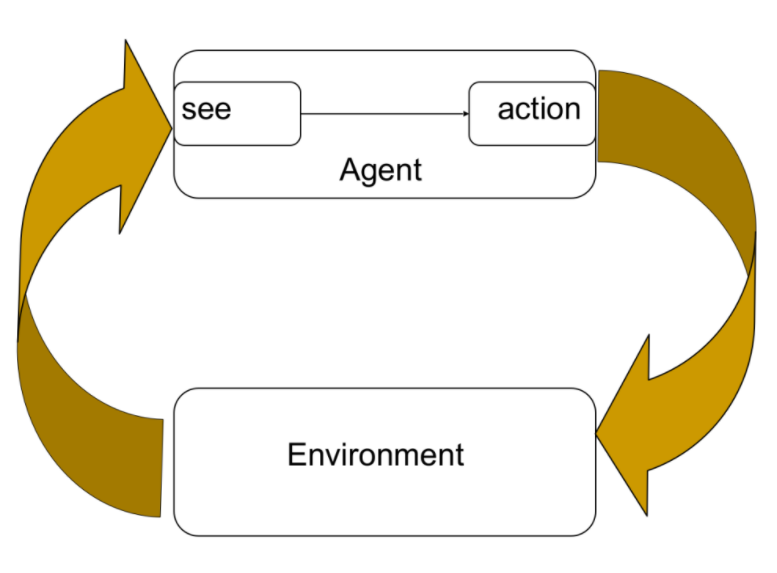
\includegraphics[scale=0.4]{images/agente reattivo.PNG}
\end{center}

\subsubsection{Agente Proattivo}
Generalmente si vuole che gli agenti siano in grado di agire \textbf{autonomamente}, quindi generare e tentare di raggiungere gli obiettivi, non solo guidati dagli eventi, ma che siano in grado di prendere l’iniziativa.

Per agire autonomamente l'agente ha bisogno di informazioni:
\begin{itemize}
    \item su come l’ambiente evolve
    \item su come le proprie azioni impattano sull’ambiente
    \item sull'obiettivo in modo tale che sia in grado di agire per raggiungerlo
\end{itemize}

Nel tentare di raggiungere un obiettivo l’agente deve essere in grado di ragionare su \textbf{piani}.

\begin{center}
    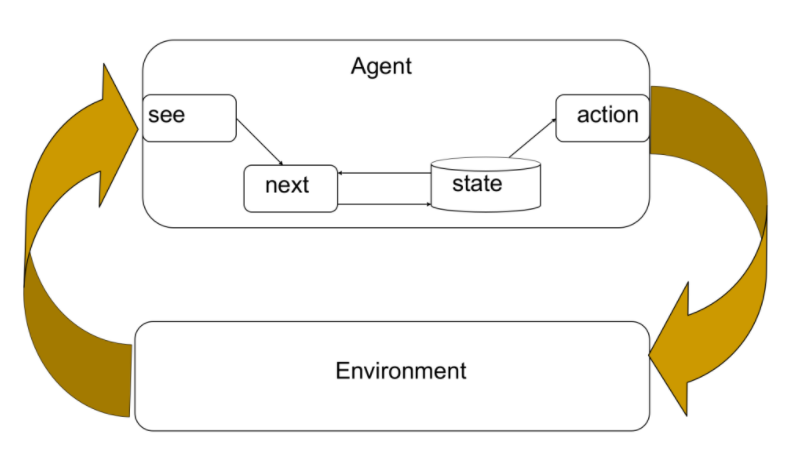
\includegraphics[scale=0.4]{images/agenti proattivi.PNG}
\end{center}

Si desidera che gli agenti siano reattivi e che rispondano ai cambiamenti per tempo e che lavorino in modo sistematico verso obiettivi di “lungo termine”, ma \textit{progettare un agente che bilanci reattività e proattività è ancora un problema di ricerca aperto}.

\subsubsection{Agente Sociale}
Per abilità sociale di un agente intelligente si intende l’abilità di interagire con altri agenti (anche umani) attraverso un qualche tipo di linguaggio di comunicazione (agent-communication language, ACL) e cooperare con essi.

\subsubsection{Conclusioni}
Un \textbf{programma non è un agente} perché il suo output non ha effetto su quello che lui percepisce in seguito e inoltre non c'è continuità temporale.

\newpage

\section{Il Triangolo della Computazione}
L'ingegneria del Software aspira a un software di qualità, quindi un software che cerca di raggiungere i seguenti goal:
\begin{itemize}
    \item Correttezza (correctness)
    \item Robustezza (robustness)
    \item Estensibilità (extensibility)
    \item Riusabilità (reusability)
\end{itemize}

Un ingrediente cruciale per raggiungere questi obiettivi è una corretta \textbf{modularizzazione} dell'architettura del software.
Il triangolo di Meyer fornisce un terreno comune per confrontare diversi approcci alla modularizzazione, dove le "forze" in gioco sono:
\begin{itemize}
    \item Process o Thread: CPU fisica, un processo o un thread.
    \item Action o Istruction: operazioni che compongono il calcolo (linguaggio macchina, operazioni fino alle subroutine).
    \item Object: strutture dati a cui le azioni si applicano.
\end{itemize}

\begin{center}
    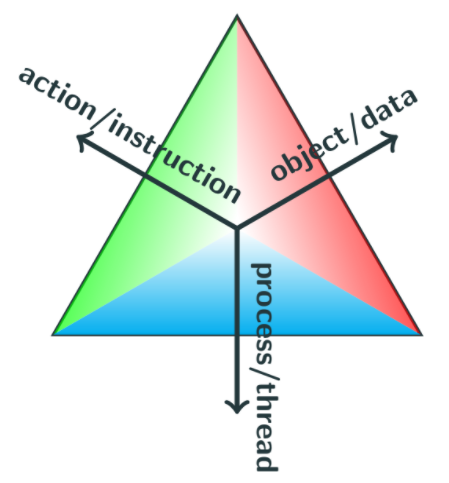
\includegraphics[scale=0.4]{images/triangolo di meyer.PNG}
\end{center}

\subsection{Decomposizione su Process o Thread}
\begin{center}
    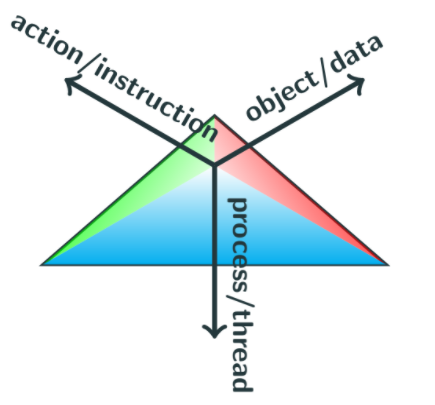
\includegraphics[scale=0.4]{images/triangolo di meyer functional.PNG}
\end{center}
\textbf{Pro}:
\begin{itemize}
    \item  Semplice ed intuitivo: decomposizione un programma in funzioni, sotto-funzioni e procedure.
    \item Algorithmic oriented: appropriato quando viene specificato un unico obiettivo principale.
\end{itemize}
\textbf{Contro}:
\begin{itemize}
    \item  Difficilmente manutenibile: difficile incorporare nuovi "obiettivi principali", quindi allo \textbf{sviluppo incrementale}.
    \item Difficilmente scalabile in presenza di dati condivisi e processi concorrenti.
\end{itemize}

\subsubsection{Business Processes}
Si tratta di un modello che crea una rappresentazione esplicita delle attività di una società/azienda e descrivere come un insieme di attività interconnesse porta a un risultato preciso e misurabile in risposta a un evento esterno.
Può essere definito come una sorta di decomposizione funzionale dove il goal si raggiunge a seguito dell'esecuzioine di un processo, diviso in sotto-processi.

Un contro è quello dovuto al fatto che l'enfasi è sul processo (vista incentrata sull'attività):
\begin{itemize}
    \item Se il dato deve influenzare il processo non funziona.
    \item Nessuna astrazione adeguata per acquisire dati manipolati lungo i flussi.
\end{itemize}

\subsection{Decomposizione su Oggetti e Dati}
\begin{center}
    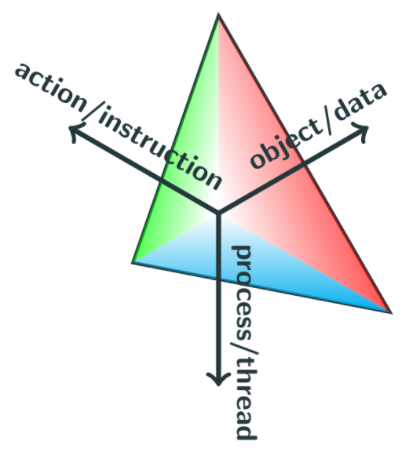
\includegraphics[scale=0.4]{images/triangolo di meyer oggetti.PNG}
\end{center}
\textbf{Pro}:
\begin{itemize}
    \item  Si adatta bene allo sviluppo incrementale, quando i requisiti non sono noti a priori.
    \item Gli oggetti hanno una vita propria, indipendente dei processi li utilizza.
    \item Operazioni sui dati: fornire le azioni di su cui è possibile operare su di essi.
\end{itemize}
\textbf{Contro}:
\begin{itemize}
    \item  Gli oggetti sono passivi: i processi esterni prendono le decisioni su quali azioni invocare oggetti.
    \item Nessun disaccoppiamento tra l'uso di un oggetto e la gestione di tale oggetto.
    \item Per la gestione dei thread si deve ovviare associando ad ogni thread un oggetto.
\end{itemize}

\subsubsection{Actors e Active Object}
Data la complessità del tentativo di coordinare gli accessi a un oggetto da più thread, a volte ha più senso evitare del tutto il multi threading e si può utilizzare il pattern degli \textbf{Actors e Active Object}. 

\textbf{Active Object} in generale è un pattern per gestire la concorrenza in cui si tenta di separare l'invocazione di un metodo dalla sua esecuzione.

Gli attori sono a un livello di astrazione più elevato rispetto a threads, infatti un \textbf{Actor} è un semplice oggetto che riceve dei messaggi e reagisce ad essi con un azione esegua sul thread corrente, quindi ad un Actor è associato il suo thread. E' possibile che l'attore decida di eseguire l'attività di azione su un pool di thread.

Uno dei problemi del modello ad attori è quello che non affronta adeguatamente il problema del coordinamento (sebbene sono state proposte estensioni). Inoltre non supporta la progettazione e la modularizzazione dei processi che utilizzano questi oggetti, perché processi esterni agli Attori.

\subsection{Il Paradigma Agent-Oriented}
La programmazione orientata agli agenti (AOP) è un paradigma di programmazione in cui la costruzione del software è centrata sul concetto di agenti software. A differenza della programmazione orientata agli oggetti che ha gli oggetti, che forniscono metodi con parametri variabili, un agente ha uno stato che è costituito da componenti come \textbf{convinzioni}, \textbf{decisioni}, capacità e \textbf{obblighi}; per questo motivo lo stato di un agente è chiamato stato mentale.

\begin{center}
    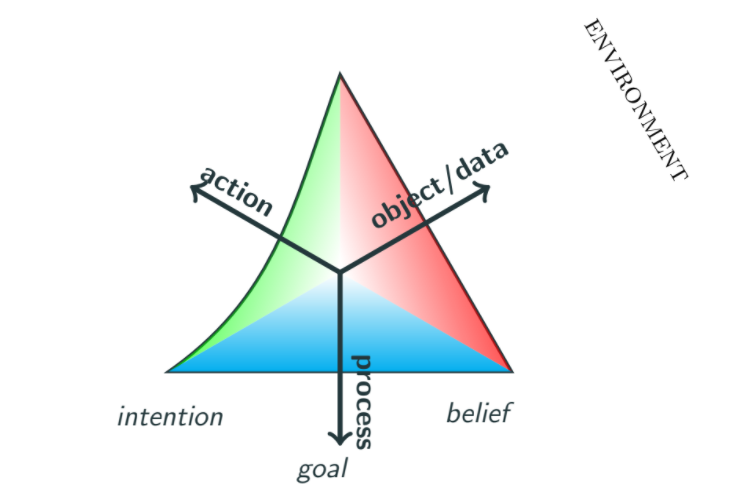
\includegraphics[scale=0.4]{images/triangolo di meyer AOP.PNG}
\end{center}
Il paradigma dell'agente si basa su due astrazioni di prima classe:
\begin{itemize}
    \item \textbf{Agenti, orientato al processo}:
        \begin{itemize}
            \item Sono autonomi, quindi il ciclo deliberativo finalizzato al raggiungimento di un obiettivo (proattività).
            \item Sono in grado di percepire e manipolare il loro ambiente.
        \end{itemize}
    \item \textbf{Ambiente, orientato ai dati/oggetto}.
\end{itemize}
Quindi per evidenziare la \textit{differenza tra Agenti e Oggetti} sottolineiamo che gli Oggetti
\begin{itemize}
    \item Non hanno il controllo sul proprio comportamento (passivo/reattivo)
    \item Non mostrano un comportamento flessibile (nessun ciclo deliberativo)
    \item Sono a thread singolo
\end{itemize}
La principale \textit{differenza tra Agenti e Attori}: Gli attori non sono intenzionali/proattivi.

\newpage

\section{Agent Architectures}
Il classico approccio per costruire agenti intelligenti è quello di vederli come casi particolare di sistemi basati sulla conoscenza, questo paradigma è noto come “symbolic AI”. 
L'architettura di un agente deliberativo, infatti, contiene una esplicita rappresentazione (modello simbolico) dell’ambiente e prende decisioni (ad esempio, quale azione eseguire) attraverso un ragionamento simbolico.

Sono due i problemi da affrontare:
\begin{itemize}
    \item Il problema della \textbf{trasduzione}: ovvero il problema della traduzione del mondo reale, dell’ambiente, in una descrizione simbolica accurata, in tempo perché sia utile (si pensi ai problemi di visione, riconoscimento del parlato, apprendimento, ...).
    \item Il problema della \textbf{rappresentazione/ragionamento}: ovvero il problema di come rappresentare simbolicamente le informazioni su entità e processi complessi del mondo reale, e come fare in modo che gli agenti ragionino con queste informazioni in tempo perché i risultati possano essere utili.
\end{itemize} 

\subsection{Agenti con ragionamento deduttivo}
Un esempio è quello del robot delle pulizie, il cui obiettivo è quello di pulire tutto lo sporco presente in un area della casa. Il primo passaggio è sicuramente quello di codificare l'ambiente, in questo caso rappresentiamo la stanza come una matrice.
\begin{center}
    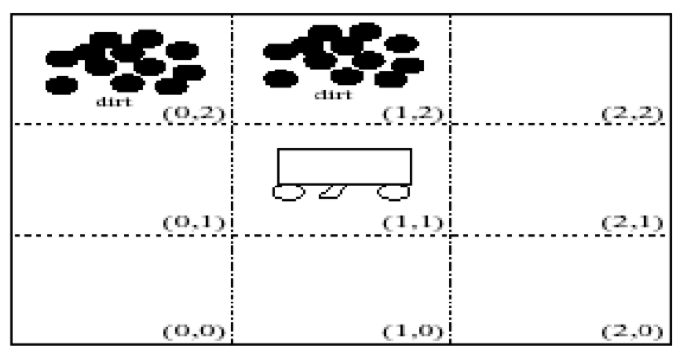
\includegraphics[scale=0.4]{images/vacuum world.PNG}
\end{center}
\textit{Ma come un agente può decidere cosa fare utilizzando tecniche di ragionamento?}

L’idea di base `e usare la logica per codificare una teoria permettendo di ottenere la migliore azione da eseguire in qualsiasi situazione.
Definiamo 3 predicati per risolvere il problema:
\begin{itemize}
    \item In(x, y), l’agente è nella posizione (x, y).
    \item Dirt(x, y), c'è dello sporco nella posizione (x, y).
    \item Facing(d), l’agente è rivolto in direzione d.
\end{itemize}
Possibili azioni: Ac = {turn, forward,suck}.
\newpage

Definiamo le regole per determinare cosa fare:
\begin{displaymath}
    In(0, 0) \land Facing(north) \land \lnot Dirt(0, 0) \Rightarrow Do(forward)
\end{displaymath}
\begin{displaymath}
    In(0, 1) \land Facing(north) \land \lnot Dirt(0, 1) \Rightarrow Do(forward)
\end{displaymath}
\begin{center}
    ...
\end{center}

Possibili \textbf{problemi} possono essere come scoprire l'ingresso della videocamera in Dirt(0, 1) e che il processo decisionale basato sulla logica del primo ordine è indecidibile.